% Prof. Dr. Ausberto S. Castro Vera
% UENF - CCT - LCMAT - Curso de Ci\^{e}ncia da Computa\c{c}\~{a}o
% Campos, RJ,  2013-2020
% Disciplina: Paradigmas de Linguagens de Programa\c{c}\~{a}o


\documentclass[12pt]{article}

% inicio do preambulo
% lista de pacotes a serem utilizados no documento
\usepackage[brazil]{babel}    % nomes e titulos em portugu\^{e}s
\usepackage[utf8]{inputenc}   % para os acentos direto do teclado
\usepackage{amsmath}          % para simbolos matem\'{a}ticos
\usepackage{here}
\usepackage{graphicx}         % para graficos e imagens
\usepackage{quoting}          % Usado em cita\c{c}\~{o}es diretas

% Prof. Dr. Ausberto S. Castro Vera
% UENF - CCT - LCMAT - Curso de Ci\^{e}ncia da Computa\c{c}\~{a}o
% Campos, RJ,  2013-2019
% Disciplina: Paradigmas de Linguagens de Programa\c{c}\~{a}o

% Arquivo: definicoes.tex


%

\usepackage{natbib}
\usepackage{hyperref}
\usepackage{xcolor}
\usepackage{tcolorbox}
\usepackage{url}

\usepackage[brazilian,hyperpageref]{backref}
% Configura\c{c}\~{o}es do pacote backref
% Usado sem a op\c{c}\~{a}o hyperpageref de backref
\renewcommand{\backrefpagesname}{Citado na(s) p\'{a}gina(s):~}
% Texto padr\~{a}o antes do n\'{u}mero das p\'{a}ginas
\renewcommand{\backref}{}
% Define os textos da cita\c{c}\~{a}o
\renewcommand*{\backrefalt}[4]{
	\ifcase #1 %
		Nenhuma cita\c{c}\~{a}o no texto.%
	\or
		Citado na p\'{a}gina #2.%
	\else
		Citado #1 vezes nas p\'{a}ginas #2.%
	\fi}%
% ---

\hypersetup{
    bookmarks=true,         % show bookmarks bar?
    unicode=false,          % non-Latin characters in Acrobat’s bookmarks
    pdftoolbar=true,        % show Acrobat’s toolbar?
    pdfmenubar=true,        % show Acrobat’s menu?
    pdffitwindow=false,     % window fit to page when opened
    pdfstartview={FitH},    % fits the width of the page to the window
    pdftitle={Modelo de Documento Simples \LaTeX},    % title
    pdfauthor={Ausberto S. Castro Vera - CC-LCMAT-CCT-UENF},     % author
    pdfsubject={Paradigmas de Linguagens de Programa\c{c}\~{a}o},   % subject of the document
    pdfcreator={ASCV, WinEdt},   % creator of the document
    pdfproducer={ASCV}, % producer of the document
    pdfkeywords={Linguagens} {LaTeX} {Documentos}, % list of keywords
    pdfnewwindow=true,      % links in new window
    colorlinks=true,       % false: boxed links; true: colored links
    linkcolor=red,          % color of internal links (change box color with linkbordercolor)
    citecolor=blue,        % color of links to bibliography
    filecolor=magenta,      % color of file links
    urlcolor=cyan           % color of external links
}	



\textwidth=15cm               % largura do texto
        % defini\c{c}\~{o}es do usu\'{a}rio

%opening
\title{\bf Modelo de Documento \\  Tipos de Refer\^{e}ncias Bibliogr\'{a}ficas \\ \texttt{plainnat}}
\author{\textsf{Prof. Ausberto S. Castro Vera} \\
	            UENF - CCT - LCMAT \\
	            Ci\^{e}ncia da Computa\c{c}\~{a}o
	   }
\date{Campos, RJ, \today}    % data. Pode ser \date{Janeiro, 2015}

\begin{document}
\maketitle     %faz o titulo usando dados do preambulo


\begin{abstract}
Este documento do tipo ARTIGO apresenta as formas b\'{a}sicas de utilizar o gerenciados JabRef e como referenciar dentro do texto as refer\^{e}ncias bibliogr\'{a}ficas que aparecem no final do texto, evitando desta maneira qualquer tipo de plagio, pirataria ou infra\c{c}\~{a}o contra os direitos autorais
\end{abstract}

\newpage
\addcontentsline{toc}{section}{Sum\'{a}rio}
\tableofcontents
\newpage

%%%%%%% ---------- Lista de arquivos do documento -----------
% Prof. Dr. Ausberto S. Castro Vera
% UENF - CCT - LCMAT - Curso de Ci\^{e}ncia da Computa\c{c}\~{a}o
% Campos, RJ,  2013-2019
% Disciplina: Paradigmas de Linguagens de Programa\c{c}\~{a}o

% Arquivo: TiposReferen.tex


\section{JabRef : Tipos de Refer\^{e}ncias Bibliogr\'{a}ficas}

JabRef (\url{http://www.jabref.org/}) \'{e} um gerenciador de refer\^{e}ncias bibliogr\'{a}ficas (c\'{o}digo aberto) que utiliza Java VM e arquivos no formato BibTeX ($\star$.bib)

\subsection{Onde pesquisar referencias bibliograficas}
\begin{itemize}
  \item Google  e Google Acad\^{e}mico (\url{https://scholar.google.com.br/})
  \item IEEE Xplore \url{http://ieeexplore.ieee.org/Xplore/home.jsp}
  \item ACM Digital Library \url{https://dl.acm.org/}
\end{itemize}


Alguns tipos de referencias bibliogr\'{a}ficas:
\begin{itemize}
  \item Livros
  \item Artigos Cient\'{\i}ficos
  \item Proceedings de Congresos
  \item Relat\'{o}rios T\'{e}cnicos (TechReport)
  \item TCC e Disserta\c{c}\~{a}o de Mestrado
  \item Teses de Doutorado
\end{itemize}


\subsection{Referencias: Livros}
\begin{itemize}
  \item Programming language concepts and paradigms, Watt (ACM Digital Library dl.acm.org) \cite{watt1990}
  \item Math into {\LaTeX}, George Gratzer \cite{Gratzer2013}
  \item Fundamentos de Seguran\c{c}a de Sistemas de Informa\c{c}\~{a}o
\end{itemize}


\subsection{Referencias:  Artigos Cient\'{\i}ficos}
\begin{itemize}
  \item 1984 Abstraction Techniques in Modern Programming Languages \cite{Shaw1984}
  \item 2010 Technical Writing Tools for Engineers and Scientists,  Cameron H.G. Wright \cite{Wright2010}
  \item 2019 Teaching Android Mobile Security \cite{Lalande2019}
\end{itemize}



\subsection{Referencias:  Proceedings - Congressos}
\begin{itemize}
  \item 2017 An Empirical Study to Revisit Productivity across Different Programming Languages
  \item 2017 An attention based image to latex markup decoder, Y. Deng and Y. Yu and J. Yao and C. Sun \cite{Deng2017}
  \item 2017 Android security issues and solutions \cite{Karthick2017}
\end{itemize}

\subsection{Relat\'{o}rios T\'{e}cnicos - TechReport}
\begin{itemize}
  \item Alessandro Warth - 2009 Experimenting with Programming Languages
  \item
\end{itemize}

% Prof. Dr. Ausberto S. Castro Vera
% UENF - CCT - LCMAT - Curso de Ci\^{e}ncia da Computa\c{c}\~{a}o
% Campos, RJ,  2013-2019
% Disciplina: Paradigmas de Linguagens de Programa\c{c}\~{a}o

% Arquivo: TiposReferen.tex


\section{Referenciando Refer\^{e}ncias Bibliogr\'{a}ficas}

Segundo o Dicion\'{a}rio Online de Portugu\^{e}s \url{https://www.dicio.com.br/plagio/}, \textbf{plagio}, \'{e} a\c{c}\~{a}o de apresentar alguma coisa (trabalho, livro, teoria etc.) como se esta fosse de sua pr\'{o}pria autoria, embora tenha sido criada e/ou desenvolvida por outrem.

Tamb\'{e}m, "o \textbf{pl\'{a}gio} (diz-se tamb\'{e}m plagiarismo ou plagiato) \'{e} o ato de assinar ou apresentar uma obra intelectual de qualquer natureza (texto, m\'{u}sica, obra pict\'{o}rica, fotografia, obra audiovisual, etc) contendo partes de uma obra que perten\c{c}a a outra pessoa sem colocar os cr\'{e}ditos para o autor original. No acto de pl\'{a}gio, o plagiador apropria-se indevidamente da obra intelectual de outra pessoa, assumindo a autoria" (\url{https://pt.wikipedia.org/wiki/Plagio}).

Ent\~{a}o \textit{evitemos o plagio} escrevendo e refer\^{e}nciando corretamente nossos trabalhos!


\subsection{Minhas ideais, minhas palavras}

 \textbf{Escrever um documento t\'{e}cnico}, entende-se, \textit{um conjunto de atividades (processo) orientadas a criar um documento de v\'{a}rias p\'{a}ginas relacionadas a uma \'{a}rea cient\'{\i}fica ou tecnol\'{o}gica. Este documento deve ter um conte\'{u}do e  uma formata\c{c}\~{a}o adequada de acordo a certas normas t\'{e}cnicas (ABNT no Brasil, por exemplo)}.

 O conte\'{u}do do par\'{a}grafo anterior n\~{a}o esta baseado especificamente em nenhuma refer\^{e}ncia. Apenas apresenta as ideias do autor sobre o que significa escrever um documento cient\'{\i}fico ou t\'{e}cnico.


\subsection{Tomando como referencia outro documento}

Segundo, \cite{Wright2010}, \textbf{escrever um documento t\'{e}cnico} \'{e} o processo de criar um documento que satisfa\c{c}a determinadas caracter\'{\i}sticas tais como: v\'{a}rias p\'{a}ginas, figuras e tabelas referenciadas no texto, se\c{c}\~{o}es l\'{o}gicas numeradas, lista de refer\^{e}ncias, lista de tabelas, lista de figuras e tabela de conte\'{u}dos (sum\'{a}rio).
\begin{figure}[H]
  \centering
  \caption{Parte do artigo original de \cite{Wright2010}}
  \includegraphics[width=12cm]{Escritatecnica.png}\\
  \textit{\small Fonte: Recorte do autor}
\end{figure}



\subsection{Tomando como referencia outros documentos}

Imagens de v\'{a}rios formatos podem ser inclu\'{\i}das em documentos \LaTeX{}. Tanto \cite{Kottwitz2011} bem como \cite{Kottwitz2015} afirmam que na inclus\~{a}o de imagens por meio de arquivos, n\~{a}o \'{e} necess\'{a}rio referenciar a extens\~{a}o do arquivo contendo a imagem (jpg, png, bmp, pdf, etc.)
\begin{figure}[H]
  \centering
  \caption{Parte dos livros de \cite{Kottwitz2011} e  \cite{Kottwitz2015}}
  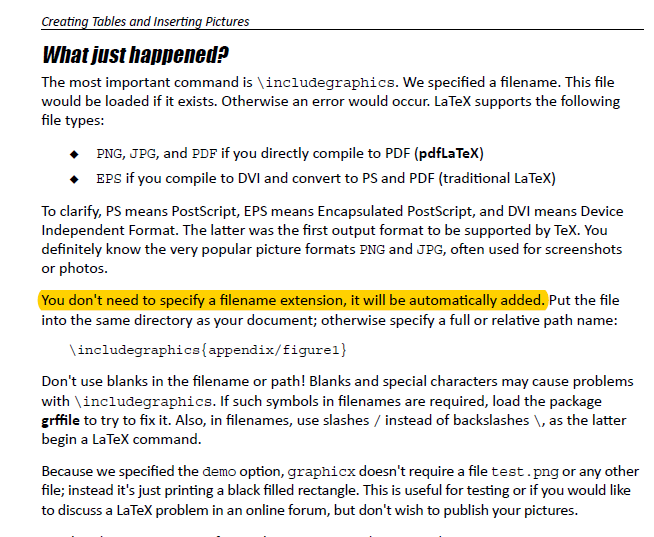
\includegraphics[width=6cm]{beginers.png}\
   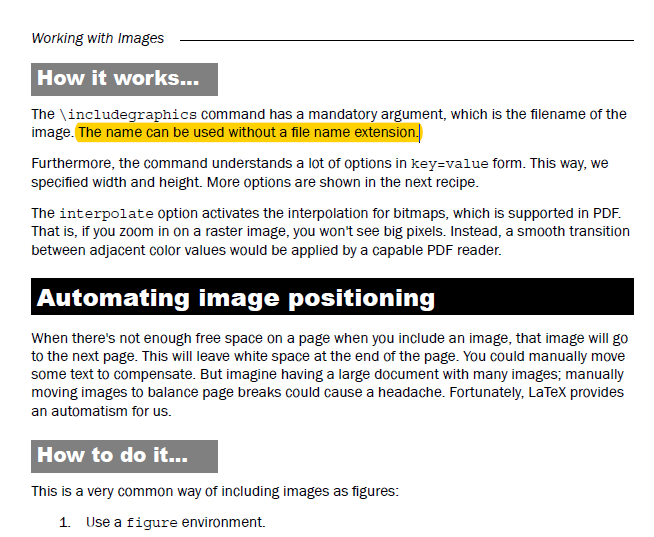
\includegraphics[width=6cm]{cookbook.png}\\
  \textit{\small Fonte: Recorte do autor}
\end{figure}

\subsection{Copiando literalmente parte de outro documento}

Utilizando as normas ABNT, as \textbf{cita\c{c}\~{o}es diretas}, no texto, com mais de tr\^{e}s linhas, devem ser destacadas com recuo de 4 cm da margem esquerda, com letra menor que a do texto utilizado e sem as aspas. A cita\c{c}\~{a}o deve ir no in\'{\i}cio ou no final da cita\c{c}\~{a}o direta. Para isto lembre-se de usar o pacote \texttt{quoting} no pre\^{a}mbulo.
\begin{verbatim}
          \usepackage{quoting}
          ....................
          \begin{document}
           ...................
          \begin{quoting}[rightmargin=0cm,leftmargin=4cm]
           \footnotesize
            .......... citacao direta AQUI .............
          \end{quoting}
\end{verbatim}

Por exemplo, uma cita\c{c}\~{a}o direta do livro de Leslie Lamport sobre o \LaTeX{}:
    \begin{quoting}[rightmargin=0cm,leftmargin=4cm] \footnotesize 
    \LaTeX{} \'{e} um sistema para tipografia de documentos. A sua primeira vers\~{a}o amplamente dispon\'{\i}vel. misteriosamente com o n\'{u}mero 2.09, apareceu em 1985. \LaTeX{} agora \'{e} extremamente popular mas comunidades cient\'{\i}ficas e acad\^{e}micas, e \'{e} utilizado extensivamente na industria. \LaTeX{} chegou a ser considerado a lingua franca (lingua de contato) do mundo cient\'{\i}fico; cientistas enviam seus papers eletronicamente para colegas ao redor do mundo na forma de arquivos \LaTeX{} \cite{lamport1994}.
    \end{quoting}
    


%%%%%%-------------------------------------------------------


%%%% Bibliografia
\addcontentsline{toc}{section}{Refer\^{e}ncias}
\bibliographystyle{plainnat}    % estilo de bibliografia
\bibliography{bibliogr, ASCVSecurity, AndroidSecurity}         % arquivo: bibliogr.bib     deve estar presente na mesma pasta

\end{document}
